
\section{Introduction \label{kugel:section:intro}}
This is the part of the book devoted to the set of functions called spherical harmonics. 
However, before we dive into the topic, we want to make a few preliminary remarks that will avoid ``upsetting'' certain types of readers. \newline
Since this is a purely mathematical topic, we felt it was appropriate to specify the mathematical style with which we will approach the various topics covered.\newline
While writing we decided to try giving demonstrations for every theorem and statement we make. However, we would like to specify that the authors of this chapter are not mathematicians and our aim is not to prove as rigorously as possible everything we say. \newline
A demonstration, to be rigorous, should consist of several simple steps using fundamental axioms. In our case, demonstrations are often not performed in this way, but rather we try to convince the reader that what we are saying stays well within the boundaries of a logical reasoning.\newline 
Sometimes we might also come across more handy demonstrations based on intuitive arguments, which can serve as intuition for the reader but would never be accepted in a mathematical context.\newline
That being said, we can get on with the interesting topics.\newline
When talking about Spherical Harmonics, one could start by describing the name. The latter could cause some confusion because of the various misleading translations into other languages, which do not fully reflect the meaning implied by the English name.\newline 
As an example, the German name for this function set is ``Kugelfunktionen'', which might imply functions defined in a spherical context, since ``Kugel'' is the german name for sphere.\newline
In contrast, the English name contains the concept of ``harmonic,'' which fits well in this context.\newline
In fact, harmonic analysis is the branch of mathematics that deals with the representation of functions using other fundamental ones, which are often easier to consider. These are called harmonics, and during the course of this chapter, you will learn that spherical harmonics belong to this class of functions, as indeed the name suggests.\newline
The structure of this chapter is organized in such a way that some mathematical concepts introduced at the beginning, will later help the reader to understand the big picture of the subject discussed.\newline
We could have performed the whole derivation without writing the chapter \ref{kugel:ssection:preleminary}. But we thought it might enhance the theory with interesting insights.\newline
The first introductory sub-chapter is devoted to the topic of vector space.\newline
In this section, vectors of finite dimensions. In addition, various mathematical operations defined in this space, including linear transformations, will be considered.\newline
We will then try to extend the concept of vectors to functions. It may sound strange that we call a function a vector, but in this context it should not be understood only in terms of its geometric sense, as we will try to explain.\newline
Having established these theoretical foundations, we may go on to the sub-chapter devoted to a well-known problem, namely, the calculation of the Eigenfunctions of the Laplace operator. This will in fact be the mathematical derivation of the spherical harmonics.\newline
This derivation will allow us to understand in a deeper way some concepts underlying the Fourier theorem, a beloved and extensively used theorem in engineering.\newline
In the third chapter we will study in more detail these special functions, defined in the previous chapter as spherical harmonics.\newline
Some of the properties we found most beautiful, interesting and useful will be thoroughly presented.\newline
To conclude this journey we decided to include some real-world applications of these functions, since being an engineer, as we are, usually means loving to make bridges between theory and practice.

\subsection{Preleminary \label{kugel:ssection:preleminary}}
The purpose of this chapter is to give a dusting off of some of the basic themes that underlie what you will read in the following subchapters.\newline
This will enable the reader to be able to get a richer view on the topic that is presented in this chapter of the book. By not limiting it to the specific example we will cover.

\subsubsection{Vector space \label{kugel:ssection:vector_space}}
A vector space, is a mathematical space in which there are entities, which we will call vectors, and some very simple rules that govern life in this world. These rules are called axioms.

Moreover, in this space, some mathematical operations are also defined, namely, addition, subtraction and linear transformations in general.\newline
The basic axioms, listed below, are responsible for ruling the behavior and interaction of these vectors.\newline
A vector space is a non-empty set $\mathcal{V}$ with a special element $\mathbf{0}$. The objects contained in this set are called vector.\newline
We can define mathematical operations as well
\begin{enumerate}
    \item \textbf{Addition}\newline
    Given two vectors $v_1, v_2 \in \mathcal{V}$, then  
    \begin{equation*}
        v_3 = v_2 + v_1 \implies v_3 \in \mathcal{V} 
    \end{equation*}

    \item \textbf{Scalar multiplication}\newline
    Given a vector $v_1 \in \mathcal{V}$ and a scalar $\alpha \in \mathbb{R}$, then  
    \begin{equation*}
        v_2 = \alpha v_1 \implies v_2 \in \mathcal{V} 
    \end{equation*}
\end{enumerate}

These operations have to satisfy the following axioms, for every $v_1,v_2,v_3 \in \mathcal{V}$ and $\alpha, \beta \in \mathbb{R}$
\begin{enumerate}
    \item \textbf{Additive axioms}
    \begin{itemize}
        \item $v_1 + v_2 = v_2 + v_1$
        \item $(v_1+v_2)+v_3 = v_1+(v_2+v_3)$
        \item $v_1 + \mathbf{0} = v_1$
        \item $v_1 + (-v_1) = \mathbf{0}$
    \end{itemize}

    \item \textbf{Multiplicative axioms}
    \begin{itemize}
        \item $\mathbf{0}v_1= v_1$
        \item $\mathbf{1}v_1 = v_1$
        \item $(\alpha \beta) v_1 = \alpha (\beta v_1)$
    \end{itemize}

    \item \textbf{Distributive axioms}
    \begin{itemize}
        \item $\alpha (v_1 + v_2) = \alpha v_1 + \alpha v_2$
        \item $(\alpha + \beta)v_1 = \alpha v_1 + \beta v_1$
    \end{itemize}
\end{enumerate}
Therefore any mathematical environment in which these rules are met can be called a vector space. 

For this sub-chapter we will use vectors in the sense of geoemetric vectors but, as written earlier this concept is not limited to geometry and can be easily extended. In the next two points we want to define two fundamental concepts present in this world, namely span and independence.

\paragraph{Span}
The span of a vector space can be seen as the set of vectors that we can build using a linear combination of the basis vectors $v_1, v_2, \hdots, v_N$.
\begin{figure}[!h]
\centering
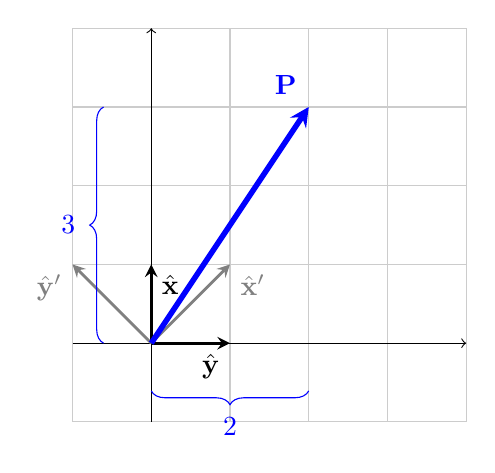
\begin{tikzpicture}
    \draw[thin,gray!40] (-1,-1) grid (4,4);
    \draw[->] (-1,0)--(4,0);
    \draw[->] (0,-1)--(0,4);
    \draw[line width=1pt,-stealth](0,0)--(0,1) node[anchor=north west]{$\hat{\mathbf{x}}$};
    \draw[line width=1pt,-stealth](0,0)--(1,0) node[anchor=north east]{$\hat{\mathbf{y}}$};
    \draw[line width=1pt, gray,-stealth](0,0)--(1,1) node[anchor=north west]{$\hat{\mathbf{x}}'$};
    \draw[line width=1pt, gray,-stealth](0,0)--(-1,1) node[anchor=north east]{$\hat{\mathbf{y}}'$};
    \draw[line width=2pt,-stealth, blue](0,0)--(2,3) node[anchor=south east]{$\mathbf{P}$};
    \draw [blue, decorate,decoration={brace, amplitude=5pt,mirror,raise=4ex}] (0,0) -- (2,0) node[midway,yshift=-3em]{2};
    \draw [blue, decorate,decoration={brace, amplitude=5pt,raise=4ex}] (0,0) -- (0,3) node[midway,xshift=-3em]{3};
\end{tikzpicture}
\caption{Example of the two basis $\{\hat{\mathbf{x}}, \hat{\mathbf{x}}\}$ and $\{\hat{\mathbf{x}}', \hat{\mathbf{y}}'\}$ with a generic vector $\mathbf{P}$. \label{fig:span}}
\end{figure}
If we consider Fig.\ref{fig:span}, an example in $\mathbb{R}^2$ can be seen. In this case, the vector $\mathbf{P}$, can in fact be constructed using a linear combination of $\hat{\mathbf{x}}$ and $\hat{\mathbf{y}}$. One can write
\begin{equation*}
    \mathbf{P} = 2\hat{\mathbf{x}} + 3\hat{\mathbf{y}}
\end{equation*}
Potentially, the vector $\mathbf{P}$, can also be represented by a combination vectors of the $\hat{\mathbf{x}}'$ and $\hat{\mathbf{y}}'$. 
We can further extend this reasoning, because any point described using $\{\hat{\mathbf{x}},\hat{\mathbf{y}}\}$, can be described using $\{\hat{\mathbf{x}}',\hat{\mathbf{y}}'\}$ as well. 
More generally, every point in $\mathbb{R}^2$ can be reached using both basis. We can therefore state that 
\begin{equation*}
    \text{span}\{\hat{\mathbf{x}},\hat{\mathbf{y}}\} = \text{span}\{\hat{\mathbf{x}}',\hat{\mathbf{y}}'\}.
\end{equation*}
This means that the span does not uniquely determine the base, but multiple bases can lead to the same span.\newline
To summarize, we can say that any vector $v_p$, belongs to a span if it can be constructed using a linear combination of its basis vectors. In mathematical terms:
\begin{equation}
    v_P \in \text{span}\{v_1,v_2, \hdots, v_N\} \iff v_P = \sum_{i=1}^N \alpha_i v_i.
\end{equation}\label{eq:def:span}
Thus, we can say that a span is the set of all the vectors that satisfy the summation in Eq.(\ref{eq:def:span}).\newline
An interesting remark is that, according to Eq.(\ref{eq:def:span}), a span always contains the $\mathbf{0}$ vector. That is beacuse by setting $\alpha_i = 0$, $\forall i$, we get $v_p=\mathbf{0}$. 

\paragraph{Independence}
If we define a span of $N$ dimensions, consisting of  $\{v_1,v_2, \hdots,v_{N}\}$, and the vector $v_N$ can be constructed using the other vectors of the span, i.e., if the vector $v_N$ does not provide any extra degrees of freedom, we can say that $v_N$ is linearly dependent, and it can be proved that
\begin{equation*}
    \text{span}\{v_1,v_2,..,v_{N-1}, v_{N}\} = \text{span}\{v_1,v_2,..,v_{N-1}\}.
\end{equation*}
Furthermore:
\begin{equation*}
    \#\text{dimensions of a span} = \#\text{linearly independent vectors}.
\end{equation*}

\paragraph{Inner product}
This operation was already introduced in the chapter \ref{}. However, in this sub-section, we wanted to recall some fundamental concepts.\newline 
So far we have only considered the operations of addition and multiplication within a vector space. However, we can now introduce a third operation, namely the inner product.\newline
In this case we will no longer speak of a simple vector space but of an \emph{inner product space}.
This new operation is simply a function that receives two vectors as input and maps them to a scalar. This mathematical operation is represented as follows
\begin{equation*}
    \langle v_1,v_2 \rangle = k, \quad k \in \mathbb{R}
\end{equation*}
The scalar product allows us to introduce some new concepts
\begin{itemize}
\item \textbf{The norm}\newline
The norm is a way to calculate the length of a vector. It can be indeed seen as a general measure for the length, that is defined as
\begin{equation*}
    ||v_p|| := \sqrt{\langle v_p,v_p \rangle}  
\end{equation*}
\item \textbf{Orthogonality}\newline
This is a concept that will be very important in the next sections.\newline 
Two vectors, $v_1$ and $v_2$, are said to be orthogonal if and only if the inner product of them is equal to zero. More formally:
\begin{equation*}
    \text{$v_1$ is orthogonal to $v_2$} \iff \langle v_1,v_2 \rangle = 0  
\end{equation*}
\end{itemize}
From the concept of orthogonality, it follows that an orthogonal basis can be defined as a set of vectors, whereby
\begin{equation*}
\{v_1,v_2,..., v_N\} \text{ is an orthogonal basis } \iff <v_n, v_m> = 0, \quad \text{if } m \neq n. 
\end{equation*}
We can also consider a more restrictive case. For example, if we are dealing with a set of orthogonal \emph{unit} vectors, we can speak of an \emph{ortonormal} basis. The conditions will then become
\begin{equation*}
\{v_1,v_2,..., v_N\} \text{ is an orthonormal basis } \iff 
\begin{cases} 
    <v_n, v_m>=0, &\text{if } m \neq n \\
    <v_n, v_m>=1, &\text{if } m = n
\end{cases}.
\end{equation*}

\paragraph{Projection of a space into a subspace}
A subspace is simply a vector space that is a subset of a larger (higher-dimensional) vector space, which is thus contained in it.\newline
For example, all vectors that are on a line passing through the origin form a subspace of $\mathbb{R}^2$. The same holds for all vectors defined on a plane passing through the origin, which itself forms a subspace of $\mathbb{R}^3$.\newline
It can be shown that a subspace is also a vector space, which can consequently be represented with an orthonormal vector span.\newline
Suppose now that we have a vector $\mathbf{P}$ in three dimensions (we still remain in the geometric context to give examples) and suppose further that we want to compute its projection in a subspace of two dimensions.\newline 
Suppose now that we have a vector P in three dimensions (we still remain in the geometric context
to give examples) and that we want to compute its projection in a subspace of two
dimensions.
In a nutshell we want to take a vector, represented with the basis vectors $\{\hat{\mathbf{x}}', \hat{\mathbf{y}}', \hat{\mathbf{z}}'\}$, and project it into the plane spanned by $\{\hat{\mathbf{x}}, \hat{\mathbf{y}}\}$.\newline
It can easily be seen that $\{\hat{\mathbf{x}}', \hat{\mathbf{y}}', \hat{\mathbf{z}}'\}$ spans $\mathbb{R}^3$. Thus we want to go from a span in three dimensions to one in two. 
\begin{figure}[!h]
\centering
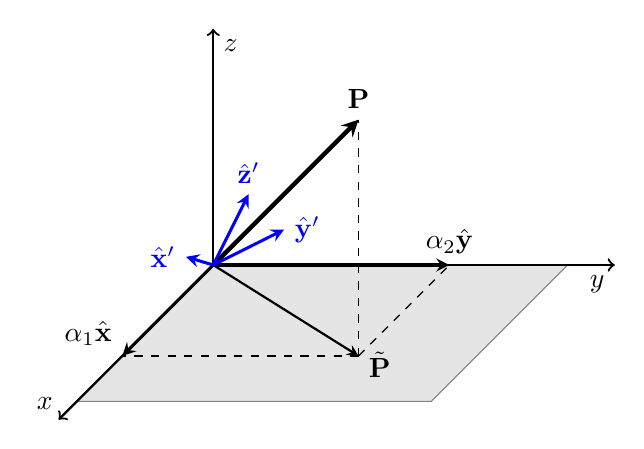
\begin{tikzpicture}[scale=3]
    \filldraw[
        draw=gray,%
        fill=gray!20,%
    ]          (0,0,0)
            -- (1.5,0,0)
            -- (1.5,0,1.5)
            -- (0,0,1.5)
            -- cycle;
    \draw[thick,->] (0,0,0) -- (1.7,0,0) node[anchor=north east]{$y$};
    \draw[thick,->] (0,0,0) -- (0,1,0) node[anchor=north west]{$z$};
    \draw[thick,->] (0,0,0) -- (0,0,1.7) node[anchor=south, xshift=-0.5em]{$x$};
    \draw[line width=1.6pt, -stealth] (0,0,0)--(1,1,1) node[anchor=south]{$\mathbf{P}$};
    \draw[line width=0.8pt, -stealth] (0,0,0)--(1,0,1) node[anchor=north west, yshift=0.5em]{$\tilde{\mathbf{P}}$};
    \draw[line width=1.1pt, -stealth] (0,0,0)--(0,0,1) node[anchor=south east]{$\alpha_1 \hat{\mathbf{x}}$};
    \draw[line width=1.1pt, -stealth] (0,0,0)--(1,0,0) node[anchor=south]{$\alpha_2 \hat{\mathbf{y}}$};
    \draw[dashed, -] (1,0,1)--(0,0,1);
    \draw[dashed, -] (1,0,1)--(1,0,0);
    \draw[dashed, -] (1,0,1)--(1,1,1);

    \draw[line width=1.1pt, -stealth, blue] (0,0,0)--(2*0.15,0.15,0) node[anchor=west]{$\hat{\mathbf{y}}'$};
    \draw[line width=1.1pt, -stealth, blue] (0,0,0)--(0,0.15,2*0.15) node[anchor=east]{$\hat{\mathbf{x}}'$};
    \draw[line width=1.1pt, -stealth, blue] (0,0,0)--(0.15,2*0.15,0) node[anchor=south]{$\hat{\mathbf{z}}'$};
\end{tikzpicture}
\caption{ \label{fig:projection_example}}
\end{figure}
If we consider Fig.(\ref{fig:projection_example}), we can visualize the problem by asking ourself: having $\mathbf{P}, \hat{\mathbf{x}}$ and $\hat{\mathbf{y}}$, how do we calculate $\alpha_1$ and $\alpha_2$?\newline
Let's say the vector $\mathbf{P}$ in $\mathbb{R}^3$ is defined as follows:
\begin{equation*}
\mathbf{P} = \alpha_1' \hat{\mathbf{x}}' + \alpha_2' \hat{\mathbf{y}}' + \alpha_3' \hat{\mathbf{z}}',
\end{equation*}
with 
\begin{align*}
    \hat{\mathbf{x}}' &= \frac{\hat{\mathbf{x}}+\hat{\mathbf{z}}}{\sqrt{2}},\\
    \hat{\mathbf{y}}' &= \frac{2\hat{\mathbf{y}}+\hat{\mathbf{z}}}{\sqrt{3}},\\
    \hat{\mathbf{z}}' &= \frac{\hat{\mathbf{y}}+2\hat{\mathbf{z}}}{\sqrt{3}}.
\end{align*}
Then, a way to project the vector $\mathbf{P}$ without knowing the coefficients of its basis vectors a priori (in this case the coefficients $\alpha_i'$) must be find.\newline
This can be done using the inner product defined above.\newline
The idea is to take $\mathbf{P}$, and project it onto the various axes we have available. Assuming that the basis we want to use in $\mathbb{R}^2$ is also orthonormal, we can write 
\begin{align*}
\tilde{\mathbf{P}} &= \langle \mathbf{P}, \hat{\mathbf{x}} \rangle  \hat{\mathbf{x}} + \langle \mathbf{P}, \hat{\mathbf{y}} \rangle  \hat{\mathbf{y}}\\
&= \alpha_1 \hat{\mathbf{x}} + \alpha_2 \hat{\mathbf{y}}
\end{align*}
In an unformal way we might say that we want to know ``how much of each axis'' is contained in $\mathbf{P}$. That is, how much information contained in $\mathbf{P}$, we can describe, using $\hat{\mathbf{x}}$ and $\hat{\mathbf{y}}$, respectively.\newline
It can be shown that the projection we obtain is the representation in fewer dimensions, which is closest to the original vector $\mathbf{P}$, meaning
\begin{equation*}
\text{min} \big\{ ||\mathbf{P}-v|| \big\} = ||\mathbf{P}-\tilde{\mathbf{P}}||,\quad v \in \text{span}\{ \hat{\mathbf{x}},\hat{\mathbf{y}} \}.
\end{equation*}

The theory just expla
ined applies to any projection of a space into its subspace. As long as the vectors of both bases are orthonormal.\newline
In the case they were orthogonal with minor adjustments the same result can be obtained.
In the most general case we can say that:\newline
a vector $\mathbf{v}$, can be represented in any orthogonal basis $\{v_1,v_2,\hdots,v_N\}$ as follows:
\begin{equation}
\mathbf{v} = \sum_{i=1}^N \alpha_i v_i
\label{eq:projection}
\end{equation}
To calculate the coefficient $\alpha_i$, we can apply a scalar product on both sides of Eq.(\ref{eq:projection}), obtaining
\begin{align*}
\langle \mathbf{v}, v_j \rangle &= \left\langle \sum_{i=1}^N \alpha_i v_i, v_j \right\rangle \\
&= \sum_{i=1}^N \langle \alpha_i v_i, v_j \rangle \\
&= \alpha_j \langle v_j, v_j \rangle \implies \alpha_i = \frac{\langle \mathbf{v}, v_j \rangle}{\langle v_i, v_i \rangle}
\end{align*}
We then have a way to represent a vector in $n$ dimensions, using fewer dimensions, in the closest possible way.

Up to this point we have not yet defined the specific operation of inner product, that is, how it is practically calculated.\newline
As written earlier the inner product is an operation that maps two vectors to a real number. It is additionally defined according to these axioms
\begin{enumerate}
\item \textbf{Linearity}
\begin{align*}
\langle \alpha v_1 + \beta v_2, v_3 \rangle &= \alpha \langle v_1, v_3 \rangle + \beta \langle v_2, v_3 \rangle \\
\langle v_1, \alpha v_2 + \beta v_3 \rangle &= \overline{\alpha} \langle v_1, v_2 \rangle + \overline{\beta} \langle v_1, v_3 \rangle
\end{align*}
\item \textbf{Conjugate Symmetry}
\begin{equation*}
\langle v_1, v_2 \rangle = \overline{ \langle v_2, v_1 \rangle}
\end{equation*}
\item \textbf{Positive-definiteness}
\begin{align*}
\langle v_1, v_1 \rangle &\geq 0 \\
\langle v_1, v_1 \rangle &= 0 \iff v_1= \mathbf{0} 
\end{align*}
\end{enumerate}
These axioms do not imply a uniqueness of the inner product. We can therefore define it as we think best.\newline
One possible definition, which meets all the axioms, in the case of vectors of finite size is the vector product, i.e.
\begin{equation*}
\langle v_1,v_2 \rangle := v_1 \cdot \overline{v_2}
\end{equation*}
We might note that when we talk about functions this operation will have to be redefined.

\subsubsection{Eigenvector \label{kugel:ssection:eigenvector}}
We do not want to spend much time on this concept, since at the bachelor's level we assume it has been explained and much used in almost all engineering fields. 
In a nutshell, an eigenvecotor of a linear transformation $\mathcal{T}\{\cdot\}$, in the context of linear algebra, is a nonzero vector that, when the linear transformation $\mathcal{T}\{\cdot\}$ is applied on it, satisfies the following equation
\begin{equation}
\mathcal{T}\{v_1\} = \lambda v_1
\label{eq:eigvec}
\end{equation}
Where $\lambda$ is called eigenvalue.\newline
Linear transformations can be viewed in general as a mapping between two vector spaces. This mapping preserves the operation of scalar multiplication and satisfies the distributive property.\newline
Recall that, if we consider a finite dimensional vector space, a linear transformation can be represented using a projection matrix, let's say $\mathbf{A}$. 
Thus, finding a vector $\mathbf{v}$, which satisfies Eq.(\ref{eq:eigvec}) is equivalent to solving the following matrix equation
\begin{equation*}
\text{det}(\mathbf{A} - \lambda \mathbf{I} ) = 0
\end{equation*}
This concept will then be extended to vector spaces of infinite dimensions in the next subsection. 

\subsubsection{Function space \label{kugel:ssection:function_space}}
Up to this point, for each example, we have considered vectors in a geometric context. However, if we consider each axiom defined above, it is very general and not at all specific, as mathematicians like.\newline
We can see that not only geometric vectors satisfy these axioms. In fact, another mathematical entity that does are functions.\newline 
So we can say that the set of all mathematical functions is a vector space.\newline
We can at least check whether this statement makes sense.\newline
Let us consider two functions $f_1(x), f_2(x)$, both with support on $\mathbb{R}$, then $f(x) = f_1(x) + f_2(x)$, still a function defined in $\mathbb{R}$.\newline 
The same is true if we multiply $f(x)$ by a constant, we remain in the space of functions defined in $\mathbb{R}$.\newline
With these two statements we have verified that the operations of sum and scalar multiplication still have the closure property. The addition, multiplication and distributive axioms can also be verified. However, we will not do that here.\newline
Therefore, the power of linear algebra allows us to consider functions as vectors. It follows that all the concepts defined earlier in \ref{kugel:ssection:vector_space} can be extended to functions.\newline
We can then have a set of basis functions, we can project functions into subspaces, have the concept of orthogonality, etc.\newline
The most famous application of this generalization of vector spaces into function spaces is probably \emph{Fourier} (at least for engineers).\newline
What is done with \emph{Fourier} is to take a function, defined in a function space with specific basis functions and project it to another basis, where the basis functions are sines and cosines. Fourier is thus a simple change of basis.

\subsubsection{Eigenfunction \label{kugel:ssection:eigenfuntion}}
As in the case of vector spaces we have the possibility of defining linear operators.\newline 
Suppose we have two vector spaces $\mathcal{A}$ and $\mathcal{B}$ (complex or real). A mapping between $\mathcal{A}$ and $\mathcal{B}$, defined as $\mathcal{T}\{\cdot\}$, is called linear if
\begin{itemize}
\item it is homogeneous, i.e:
\begin{equation*}
    \mathcal{T}\{\lambda x\} = \lambda \mathcal{T}\{x\},
\end{equation*}
\item it is additive, i.e:
\begin{equation*}
    \mathcal{T}\{x+y\} = \mathcal{T}\{x\}+\mathcal{T}\{y\}.
\end{equation*}
\end{itemize}
In the case of finite-dimensional vector spaces, as written earlier, we can consider these linear transformations as matrices, in fact we can map, for example, a vector space $\mathbb{R}^n$ onto $\mathbb{R}^m$, using a matrix of dimension $n \times m$.\newline
However, we can define operators for vector spaces of infinite dimensions (in this case, function spaces) too.\newline
For example, the derivative is an operator that maps functions from $C^1\to C$, where $C^1$ is the set of all once differentiable functions and $C$ denotes the set of continuous and real functions.\newline
In the case of operators defined in finite-dimensional vector spaces, we can compute eigenvectors. In function spaces we have mathematical objects with the same properties, we will refer to them as \emph{eigenfunctions}.\newline 
An eigenfunction of an operator $\mathcal{T}\{\cdot\}$, analogous to the eigenvector, is a function that satisfies the following equation:
\begin{equation*}
\mathcal{T}\{f(x)\} = \lambda f(x).
\end{equation*}
A couple of examples are
\begin{itemize}
\item For the differential operator $\dfrac{d}{dx}\{\cdot\}$, the function $e^{ax}$ is an eigenfunction.
\item For the fourier operator $\mathcal{F}\{\cdot\}$, the \emph{Gaussian function} $e^{-\frac{(x-\mu)^2}{2\sigma^2}}$.
\item $\hdots$
\end{itemize}
Another example of a linear operator is the \emph{Laplace operator} $\nabla^2$, which is very important in engineering and mathematics. Its eigenfunctions will not be discussed in this subsection because the next section is devoted entirely to them. 